%%%%%%%%%%%%%%%%%%%%%%%%%%%%%%%%%%%%%%%%%%%%%%%%%%%%%%%%
% Este é um documento que servirá de modelo para
% os relatórios feitos na disciplina Circuitos Digitais
% 2016-2
%%%%%%%%%%%%%%%%%%%%%%%%%%%%%%%%%%%%%%%%%%%%%%%%%%%%%%%%%

\PassOptionsToPackage{brazil,american}{babel}
\documentclass[12pt]{article}

\usepackage{sbc-template}
\usepackage[brazil,american]{babel}
\usepackage[utf8]{inputenc}

\usepackage{graphicx}
\usepackage{url}
\usepackage{float}
\usepackage{listings}
\usepackage{color}
\usepackage{todonotes}
\usepackage{algorithmic}
\usepackage{algorithm}
\usepackage{hyperref}
     
\sloppy

\title{Experimento 7\\ 
Circuitos Combinacionais: Multiplexadores}

\author{Lucas Mafra Chagas, 12/0126443\\
        Marcelo Giordano Martins Costa de Oliveira,  12/0037301\\
}


\address{Dep. Ciência da Computação -- Universidade de Brasília (UnB)\\
  CiC 116351 - Circuitos Digitais - Turma A
  \email{\{giordano.marcelo, chagas.lucas.mafra\}@gmail.com}
}

\begin{document} 

\maketitle

 \begin{abstract}
   Write here a short summary of the report in English. This corresponds to the Experiment 7 report on combinational circuits, specifically the multiplexers.
 \end{abstract}
     
 \begin{resumo} 
  Escreva aqui um pequeno resumo do relatório. Este corresponde ao relatório do Experimento 7 sobre circuitos combinacionais, especificamente os multiplexadores.
 \end{resumo}


\section{Objetivos}
\label{sec:Objetivos}

Fornecer ao aluno um contato inicial com o painel. São apresentadas as portas AND, OR e
NOT e os conceitos de atraso em portas lógicas e nível de ruído em circuitos digitais.

\section{Materiais} 
\label{sec:Materiais}

\begin{itemize}
    \item Painel Digital;
    
    \item \textit{protoboard};
    
    \item Fios conectores;
    
    \item Portas lógicas AND (7408), OR(7432) e NOT(7404);
    
    \item Fios conectores;
    
    \item Multímetro;
    
    \item Ponta lógica;
    
\end{itemize}


\section{Introdução}
\label{sec:Introducao}

Escreva com suas palavras o que vai ser trabalhado no experimento. Aqui temos um exemplo de como citar a bibliografia consultada \cite{boulic:91} \cite{smith:99}.

\section{Procedimentos}
\label{sec:Procedimentos}

Escreva nesta seção os diversos itens pedidos no experimentos. 

\subsection{Funcionamento das portas lógicas AND e OR}
\label{sec:Porta Lógica}


\begin{table}
	\centering
	\begin{tabular}{|c|c|c|c|c|c|c|c|}
	\cline{1-6}
	\multicolumn{1}{|c|}{A} & \multicolumn{1}{|c|}{B} & \multicolumn{1}{|c|}{S1} & \multicolumn{1}{|c|}{S2} & \multicolumn{1}{|c|}{S3} & \multicolumn{1}{|c|}{S4}\\
	\hline
	0 & 0 & 0.01 & 0.02 & 0.02 & 0.02\\
	0 & 1 & 0.01 & 0.02 & 0.02 & 0.02\\
	1 & 0 & 0.01 & 0.02 & 0.02 & 0.02\\
	1 & 1 & 4.99 & 4.98 & 4.96 & 4.97\\
	\hline
	\end{tabular}
	\label{Porta AND}
\end{table}

\begin{table}
	\centering
	\begin{tabular}{|c|c|c|c|c|c|c|c|}
	\cline{1-6}
	\multicolumn{1}{|c|}{A} & \multicolumn{1}{|c|}{B} & \multicolumn{1}{|c|}{S1} & \multicolumn{1}{|c|}{S2} & \multicolumn{1}{|c|}{S3} & \multicolumn{1}{|c|}{S4}\\
	\hline
	0 & 0 & 0.03 & 0.01 & 0.01 & 0.05\\
	0 & 1 & 4.98 & 4.97 & 4.98 & 4.98\\
	1 & 0 & 4.98 & 4.97 & 4.97 & 4.98\\
	1 & 1 & 4.98 & 4.97 & 4.97 & 4.97\\
	\hline
	\end{tabular}
	\label{Porta OR}
\end{table}

Descrever o experimento realizado. Sempre  que colocar uma figura deve-se explicar o que se pretende que o leitor veja, ou uma análise logo após a figura. 


Aqui temos um exemplo de como citar uma URL na bibliografia~\cite{systemverilog}.


É apresentado acima como fazer uma listagem não numerada.

\subsection{Implementação da porta OR com portas AND e NOT}
\label{sec:NOTAND}

\begin{figure}[H]
\centering
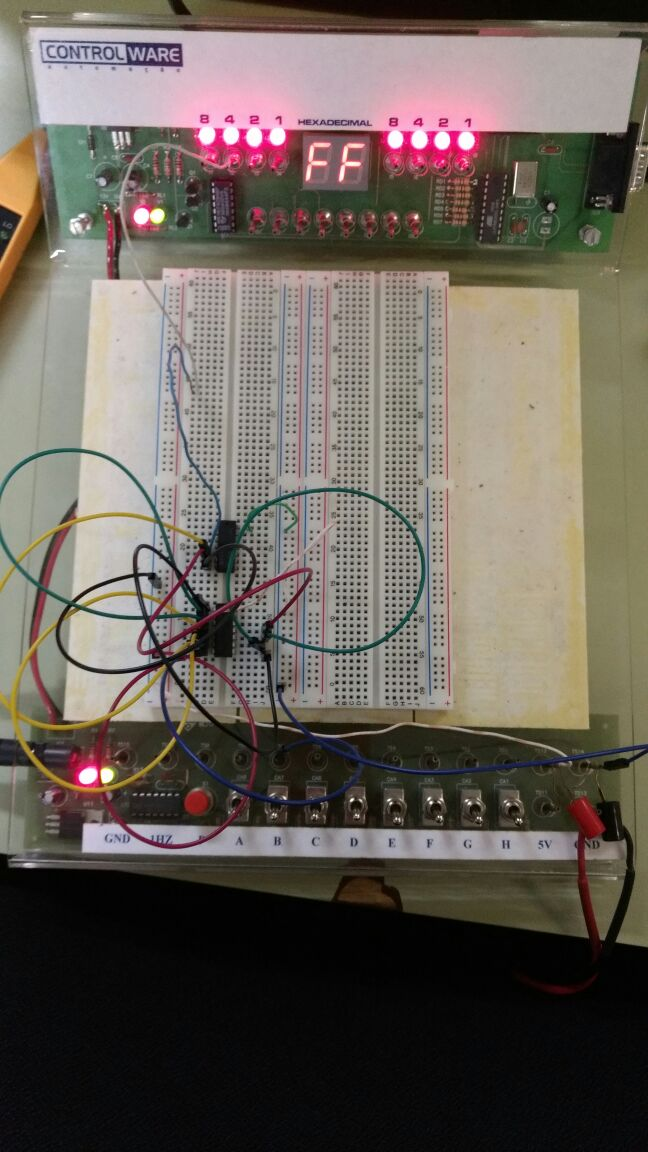
\includegraphics[width=.5\textwidth]{Porta_OR.jpeg}
\caption{Uma figura}
\label{fig:portaor}
\end{figure}

A Figura~\ref{fig:portaor} apresenta um exemplo de como usar e citar uma figura.

\begin{table}
	\centering
	\begin{tabular}{|c|c|c|c|}
	\cline{1-4}
	\multicolumn{1}{|c|}{A} & \multicolumn{1}{|c|}{B} & \multicolumn{1}{|c|}{S1}\\
	\hline
	0 & 0 & 0\\
	0 & 1 & 1\\
	1 & 0 & 1\\
	1 & 1 & 1\\
	\hline
	\end{tabular}
	\label{Porta OR}
\end{table}



\subsection{Implementação da porta AND com portas OR e NOT}
\label{sec:NOTOR}

\begin{figure}[H]
\centering
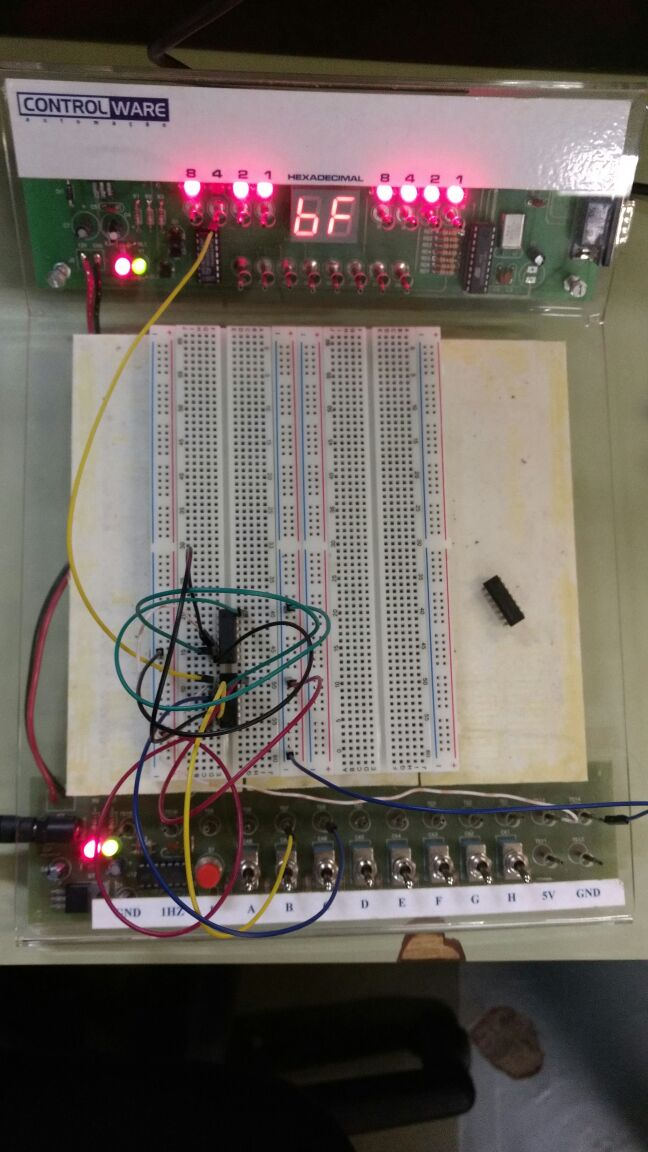
\includegraphics[width=.5\textwidth]{Porta_AND.jpeg}
\caption{Uma figura}
\label{fig:portaand}
\end{figure}

A Figura~\ref{fig:portaand} apresenta um exemplo de como usar e citar uma figura.

\begin{table}
	\centering
	\begin{tabular}{|c|c|c|c|}
	\cline{1-4}
	\multicolumn{1}{|c|}{A} & \multicolumn{1}{|c|}{B} & \multicolumn{1}{|c|}{S1}\\
	\hline
	0 & 0 & 0\\
	0 & 1 & 0\\
	1 & 0 & 0\\
	1 & 1 & 1\\
	\hline
	\end{tabular}
	\label{Porta OR}
\end{table}

\subsection{Atraso de Propagação em Portas}
\label{sec:atraso}

Aqui temos um exemplo de como criar um hiperlink. Veja
\href{https://www.youtube.com/watch?v=EcNxjxKRQ6E}{aqui} um exemplo de vídeo.

Sempre identifique no site do vídeo:
\begin{itemize}
    \item o experimento: Experimento 7;
    \item semestre: 2016-2;
    \item a disciplina: CiC 116351 - Circuitos Digitais - Turma B;
    \item a universidade: Universidade de Brasília (UnB);
    \item os nomes dos componentes do grupo.
\end{itemize}

\section{Análise dos Resultados}
\label{sec:Resultados}

Faça uma análise crítica dos resultados obtidos nos experimentos. Esta análise pode ser feita item a item ou de uma forma geral.

Dica: Use pesquisa na Internet para tirar as dúvidas sobre edição em \LaTeX .

\section{Conclusão}
\label{sec:Conclusao}

Concluir o relatório explanando rapidamente o que foi feito e os resultados obtidos, sempre correlacionando com os objetivos do experimento apresentado na Seção~\ref{sec:Objetivos}. 


\bibliographystyle{sbc}
\bibliography{relatorio}


\newpage 
% Colocar aqui apenas as respostas dos itens da Auto-Avaliação
\section*{Auto-Avaliação}

\begin{enumerate}
    \item a
    \item c
    \item b
    \item d
\end{enumerate}


\end{document}
